\documentclass[11pt,a4paper]{article}

\usepackage{fontspec}
\usepackage{xeCJK}
\usepackage{geometry}
\usepackage{graphicx}
\usepackage{booktabs}
\usepackage{tabularx}
\usepackage{array}
\usepackage{xcolor}
\usepackage{hyperref}
\usepackage{enumitem}
\usepackage{caption}
\usepackage{fancyhdr}
\usepackage{titlesec}

\geometry{left=24mm,right=24mm,top=24mm,bottom=26mm}
\setmainfont{DejaVu Sans}
\setsansfont{DejaVu Sans}
\setmonofont{DejaVu Sans Mono}
\setCJKmainfont{Noto Serif CJK SC}
\setCJKsansfont{Noto Sans CJK SC}
\setCJKmonofont{Noto Sans CJK SC}

\definecolor{reportInk}{HTML}{172033}
\definecolor{reportMuted}{HTML}{5B6472}
\definecolor{reportAccent}{HTML}{2563EB}
\definecolor{reportAccentDark}{HTML}{1D4ED8}
\definecolor{reportSoft}{HTML}{EFF6FF}
\definecolor{reportLine}{HTML}{BFDBFE}

\hypersetup{
  colorlinks=true,
  linkcolor=reportAccentDark,
  urlcolor=reportAccentDark,
  citecolor=reportAccentDark,
  pdftitle={家庭电力消耗多步预测机器学习课程大作业},
  pdfauthor={ML Homework}
}

\graphicspath{{../results/official_summary/figures/}{results/official_summary/figures/}}
\setlength{\parindent}{2em}
\setlength{\parskip}{0.35em}
\setlength{\headheight}{23pt}
\renewcommand{\arraystretch}{1.18}
\renewcommand{\contentsname}{目录}
\renewcommand{\figurename}{图}
\renewcommand{\tablename}{表}
\captionsetup{font=small,labelfont={bf,color=reportAccentDark}}

\pagestyle{fancy}
\fancyhf{}
\lhead{\sffamily\small 家庭电力消耗多步预测}
\rhead{\sffamily\small 机器学习课程大作业}
\cfoot{\sffamily\small\thepage}
\renewcommand{\headrulewidth}{0.4pt}
\renewcommand{\headrule}{\hbox to\headwidth{\color{reportLine}\leaders\hrule height \headrulewidth\hfill}}

\titleformat{\section}
  {\Large\sffamily\bfseries\color{reportAccentDark}}
  {\thesection}{0.7em}{}
\titleformat{\subsection}
  {\large\sffamily\bfseries\color{reportInk}}
  {\thesubsection}{0.7em}{}
\titlespacing*{\section}{0pt}{1.6em}{0.7em}
\titlespacing*{\subsection}{0pt}{1.1em}{0.45em}

\newcommand{\metric}[2]{#1\,{\footnotesize$\pm$\,#2}}
\newcommand{\pill}[1]{\textcolor{reportAccentDark}{\sffamily\bfseries #1}}

\begin{document}

\begin{titlepage}
  \thispagestyle{empty}
  \vspace*{0.4cm}
  {\sffamily\bfseries\fontsize{25}{31}\selectfont 家庭电力消耗多步预测\\机器学习课程大作业\par}
  \vspace{0.8cm}
  {\Large\sffamily\color{reportAccentDark} LSTM、Transformer 与 LSTM+Transformer Ensemble 对比实验\par}
  \vspace{1.1cm}

  \begin{center}
  {\setlength{\fboxsep}{8pt}\colorbox{reportSoft}{%
    \begin{minipage}{0.88\textwidth}
      \vspace{0.6em}
      \sffamily
      \begin{tabularx}{\linewidth}{@{}>{\bfseries\color{reportAccentDark}}l X@{}}
        任务 & 基于过去 90 天多变量电力消耗序列，预测未来 90 天与 365 天每日 \texttt{global\_active\_power}。\\
        数据集 & UCI Machine Learning Repository: Individual household electric power consumption。\\
        指标 & 测试集 MSE 与 MAE，报告 5 个 seed 的 mean $\pm$ std，数值位于标准化目标尺度。\\
        最终模型 & 固定 0.5/0.5 权重的 LSTM+Transformer Ensemble。\\
        仓库 & \href{https://github.com/ziangbuchu/ML_homework}{GitHub 仓库}\\
      \end{tabularx}
      \vspace{0.6em}
    \end{minipage}%
  }}
  \end{center}

  \vfill
  \noindent{\sffamily\color{reportMuted} 本报告按单人作业组织，未涉及组队贡献拆分。所有表格与图像来自仓库中正式实验产物 \texttt{results/official\_summary/}。}
\end{titlepage}

\tableofcontents
\newpage

\section{问题介绍}

家庭电力消耗预测是典型的多变量时间序列回归问题。给定一段历史用电观测，需要估计未来一段时间的总有功功率变化。该问题同时具有短期局部波动、周期性变化和长期趋势不确定性，因此适合比较循环神经网络、Transformer 和结构改进模型在不同预测跨度上的表现。

本项目使用 UCI 公开的 Individual household electric power consumption 数据集，页面为 \href{https://archive.ics.uci.edu/dataset/235/individual+household+electric+power+consumption}{UCI 数据集页面}。原始数据覆盖 2006-12-16 至 2010-11-26 的分钟级家庭电力观测，共 2,075,259 条记录。数据字段包括 \texttt{global\_active\_power}、\texttt{global\_reactive\_power}、\texttt{voltage}、\texttt{global\_intensity}、三个 sub-metering 分量，以及由总功率和分项功率推导得到的 remainder 分量。清洗时先按分钟时间轴补齐索引，对缺失分钟做时间插值并前后填充，再聚合为 1,442 条日级样本。

实验输入窗口固定为 90 天，输出窗口分别为 90 天和 365 天。为了保证长期预测也有足够验证和测试样本，本项目按滑动窗口样本做时间顺序切分：90 天输出共有 1,263 个窗口，train/val/test 为 884/189/190；365 天输出共有 988 个窗口，train/val/test 为 691/148/149。所有模型使用同一数据流水线、同一指标定义和同一结果记录格式。

\subsection{实验设计取舍}

本实验没有把时间序列问题简化为随机打散的普通回归任务，而是保留时间顺序切分。这样做牺牲了一部分训练样本的随机性，但能更接近真实预测场景：模型只能利用较早时间段学习，并在较晚时间段接受测试。由于滑动窗口之间仍存在相邻重叠，报告中的 test 指标更适合解释为同一住户时间序列上的 out-of-sample 预测能力，而不是完全独立住户或完全独立年份上的泛化能力。

输入窗口固定为 90 天，是对数据规模和预测难度的折中。窗口太短会削弱季节性和月度用电模式，窗口太长则会显著减少可用训练窗口，尤其会压缩 365 天预测任务的验证/测试样本。输出同时设置 90 天与 365 天，是为了区分短期局部波动预测和长期趋势预测：前者更依赖近期状态记忆，后者更考验模型是否能学到跨季节的平滑趋势。

指标在标准化目标尺度上计算，主要用于公平比较模型，而不是直接报告电力工程意义上的 kW 误差。这个选择避免了不同 horizon 下目标幅度差异干扰模型排序，但也意味着结论边界必须保持清楚：本文支持的是模型相对优劣，不直接声称绝对用电量误差已经满足部署要求。

\section{模型}

本项目实现 LSTM、Transformer 两类 baseline，并在多次尝试后采用 LSTM+Transformer Ensemble 作为最终改进模型。另保留 TCN+Transformer 作为一次结构改进尝试和负结果对照。

\subsection{模型归纳偏置与风险}

三类结构的核心差别不是“谁更复杂”，而是各自默认相信什么模式。LSTM 的递归状态天然偏向连续时间记忆，适合小数据下捕捉局部演化，但长期预测时容易把未来压缩到单个隐藏向量中。Transformer 的自注意力更擅长直接比较输入窗口内任意两天的关系，长期 horizon 上更灵活，但在样本较少时也更容易学到不稳定的全局相关。TCN+Transformer 原本希望用卷积先抽取局部波动、再交给注意力建模全局关系；它失败的原因可能不是“卷积无用”，而是当前日级样本量、训练轮数和输出跨度不足以支持额外结构带来的优化成本。

最终 ensemble 的出发点是风险分散而不是堆叠复杂度。LSTM 与 Transformer 在两个 horizon 上表现互补，等权平均相当于把两种错误模式做线性折中：如果单模型误差不是完全同向，平均预测就可能降低方差和局部偏差。为了避免把测试集变成调参集，ensemble 权重固定为 0.5/0.5，不在测试集上搜索最优权重。

\subsection{LSTM 基线}

LSTM 基线将 90 天输入序列编码为隐藏状态，再用最后一个隐藏状态直接投影到完整预测窗口。该模型的优势是参数量较小、对时间顺序建模直接，适合验证在小规模日级数据上的稳健性。

\begin{center}
\begin{minipage}{0.82\textwidth}
\begin{verbatim}
Input X: [batch, 90, feature_dim]
H = LSTM(X)
z = H_last
y_hat = Linear(z) -> [batch, horizon]
\end{verbatim}
\end{minipage}
\end{center}

\subsection{Transformer 基线}

Transformer 基线先将输入特征投影到 \texttt{d\_model} 维空间，加入正弦位置编码，再通过 Transformer Encoder 建模日级序列中的全局依赖。Encoder 输出经过时间维平均池化后，投影为未来 90 天或 365 天预测。

\begin{center}
\begin{minipage}{0.82\textwidth}
\begin{verbatim}
E = Linear(X) + SinusoidalPositionEncoding
Z = TransformerEncoder(E)
z = MeanPool(Z, time)
y_hat = Linear(z) -> [batch, horizon]
\end{verbatim}
\end{minipage}
\end{center}

\subsection{改进模型：LSTM+Transformer Ensemble}

初始改进尝试为 TCN+Transformer，即在 Transformer 前加入残差 temporal convolution block，以提取局部用电波动。但正式五轮结果显示该结构在 90 天和 365 天上均未超过 baseline。进一步分析发现，LSTM 在短期预测上更稳，而 Transformer 在长期预测上更强，因此最终改进模型采用固定等权重 ensemble，直接融合两种归纳偏置。

\begin{center}
\begin{minipage}{0.82\textwidth}
\begin{verbatim}
y_lstm = LSTM(X)
y_transformer = Transformer(X)
y_hat = 0.5 * y_lstm + 0.5 * y_transformer
\end{verbatim}
\end{minipage}
\end{center}

ensemble 权重固定为 0.5/0.5，没有按测试集调参。脚本会加载同一 seed 下已训练的 LSTM 和 Transformer 权重，重新评估 train/val/test 三个 split，并生成 ensemble 的 \texttt{metrics.json}、\texttt{predictions\_test.npz} 和预测曲线图。LSTM、Transformer 和 TCN+Transformer 训练使用 Adam 优化器，学习率 1e-3，batch size 32，最多 8 epochs，early stopping patience 3。

\section{结果与分析}

正式实验包含 30 次神经网络训练运行，以及 10 次 ensemble 评估运行。汇总脚本从正式 run 目录收集每个 seed 的 train/val/test 指标，并在报告汇总目录下生成 by-run 明细、summary 汇总和报告表格。表 \ref{tab:results} 列出测试集结果。

除神经网络模型外，本项目还补充了两个 deterministic naive baseline：\texttt{last\_value} 将输入窗口最后一天的标准化目标值重复到整个预测窗口，\texttt{input\_mean} 将输入窗口目标均值重复到未来。它们不参与最终模型竞争，只用于检查神经网络是否确实超过简单持久性预测。测试集上，\texttt{input\_mean} 在 90/365 天的 MSE 分别为 0.736495/1.036502，\texttt{last\_value} 分别为 0.923572/1.431294，均明显弱于 LSTM+Transformer Ensemble。

\begin{table}[htbp]
\centering
\caption{正式测试集 5 seed mean $\pm$ std 对比。最优结果为 LSTM+TF Ensemble。}
\label{tab:results}
\small
\begin{tabularx}{\textwidth}{@{}l r >{\raggedleft\arraybackslash}X >{\raggedleft\arraybackslash}X r@{}}
\toprule
Model & Horizon & Test MSE mean$\pm$std & Test MAE mean$\pm$std & n \\
\midrule
LSTM & 90 & \metric{0.461748}{0.025748} & \metric{0.528486}{0.016241} & 5 \\
\pill{LSTM+TF Ensemble} & 90 & \pill{\metric{0.374844}{0.021490}} & \pill{\metric{0.476894}{0.012026}} & 5 \\
TCN+Transformer & 90 & \metric{0.512452}{0.028040} & \metric{0.579678}{0.016588} & 5 \\
Transformer & 90 & \metric{0.471832}{0.023400} & \metric{0.554246}{0.021258} & 5 \\
\midrule
LSTM & 365 & \metric{0.499038}{0.096153} & \metric{0.550961}{0.058222} & 5 \\
\pill{LSTM+TF Ensemble} & 365 & \pill{\metric{0.444566}{0.034877}} & \pill{\metric{0.516384}{0.022741}} & 5 \\
TCN+Transformer & 365 & \metric{0.655113}{0.071301} & \metric{0.638373}{0.036456} & 5 \\
Transformer & 365 & \metric{0.463998}{0.036387} & \metric{0.526030}{0.023207} & 5 \\
\bottomrule
\end{tabularx}
\end{table}

90 天预测中，LSTM+Transformer Ensemble 的测试 MSE 和 MAE 均最低。相对最强单模型 LSTM，ensemble 的 MSE 从 0.461748 降至 0.374844，约下降 18.82\%；MAE 从 0.528486 降至 0.476894，约下降 9.76\%。这说明短期任务中 LSTM 的局部记忆仍然重要，但 Transformer 的补充信息能进一步修正部分系统性偏差。

365 天预测中，Transformer 是最强单模型，但 LSTM+Transformer Ensemble 继续取得最低测试 MSE 和 MAE。相对 Transformer，ensemble 的 MSE 约下降 4.19\%，MAE 约下降 1.83\%。长期任务的提升幅度小于短期任务，说明长期趋势误差更难通过简单平均完全消除，但等权融合仍然带来了稳定收益。

TCN+Transformer 是本项目中有价值的负结果。它在两个窗口上均未超过 baseline，提示“增加局部卷积模块”并不自动带来更好的时间序列预测。结合数据规模看，额外卷积层可能放大了优化难度，也可能把有限样本中的局部噪声当成稳定模式。保留这一负结果可以避免只汇报成功模型导致的选择性叙述。

\subsection{Ensemble 权重选择消融}

为了检验固定 0.5/0.5 权重是否只是偶然选择，本项目进一步补充了 ensemble weight sweep。对每个 horizon 和 seed，在 $\{0.0, 0.1, \ldots, 1.0\}$ 上扫描 LSTM 权重，并且只允许用验证集 MSE 选择权重；测试集最优权重只作为 diagnostic oracle 报告，不参与模型选择。该实验由 \path{scripts/run_ensemble_weight_sweep.py} 生成，产物位于 \path{results/official_summary/ensemble_weight_summary.md}。

\begin{table}[htbp]
\centering
\caption{LSTM+Transformer ensemble 权重选择消融。Test-oracle 仅用于诊断，不用于选择最终模型。}
\label{tab:weight-sweep}
\small
\begin{tabularx}{\textwidth}{@{}r l >{\raggedleft\arraybackslash}X >{\raggedleft\arraybackslash}X@{}}
\toprule
Horizon & Rule & Test MSE mean$\pm$std & Test MAE mean$\pm$std \\
\midrule
90 & equal 0.5 & \metric{0.374842}{0.021491} & \metric{0.476893}{0.012027} \\
90 & validation-selected & \metric{0.446209}{0.043318} & \metric{0.518641}{0.027420} \\
90 & test-oracle diagnostic & \metric{0.374186}{0.021537} & \metric{0.475724}{0.011638} \\
\midrule
365 & equal 0.5 & \metric{0.444563}{0.034875} & \metric{0.516382}{0.022740} \\
365 & validation-selected & \metric{0.442416}{0.017311} & \metric{0.513660}{0.010671} \\
365 & test-oracle diagnostic & \metric{0.429071}{0.012882} & \metric{0.504761}{0.008479} \\
\bottomrule
\end{tabularx}
\end{table}

消融结果说明，最终不应简单把“验证集调权”替换为主模型。90 天任务中，验证集选择的权重多为 0.7 或 1.0，即明显偏向 LSTM；但测试集上反而显著劣于 equal 0.5，说明验证集和测试集在短期窗口上存在一定分布差异。365 天任务中，验证集调权略优于 equal 0.5，说明长期预测可以从 horizon-specific 权重中获益。综合两个 horizon，固定等权重不是最激进的选择，但它避免了按验证集过度适配某一窗口，在当前课程作业设置下更稳健、更容易解释。

\begin{figure}[htbp]
  \centering
  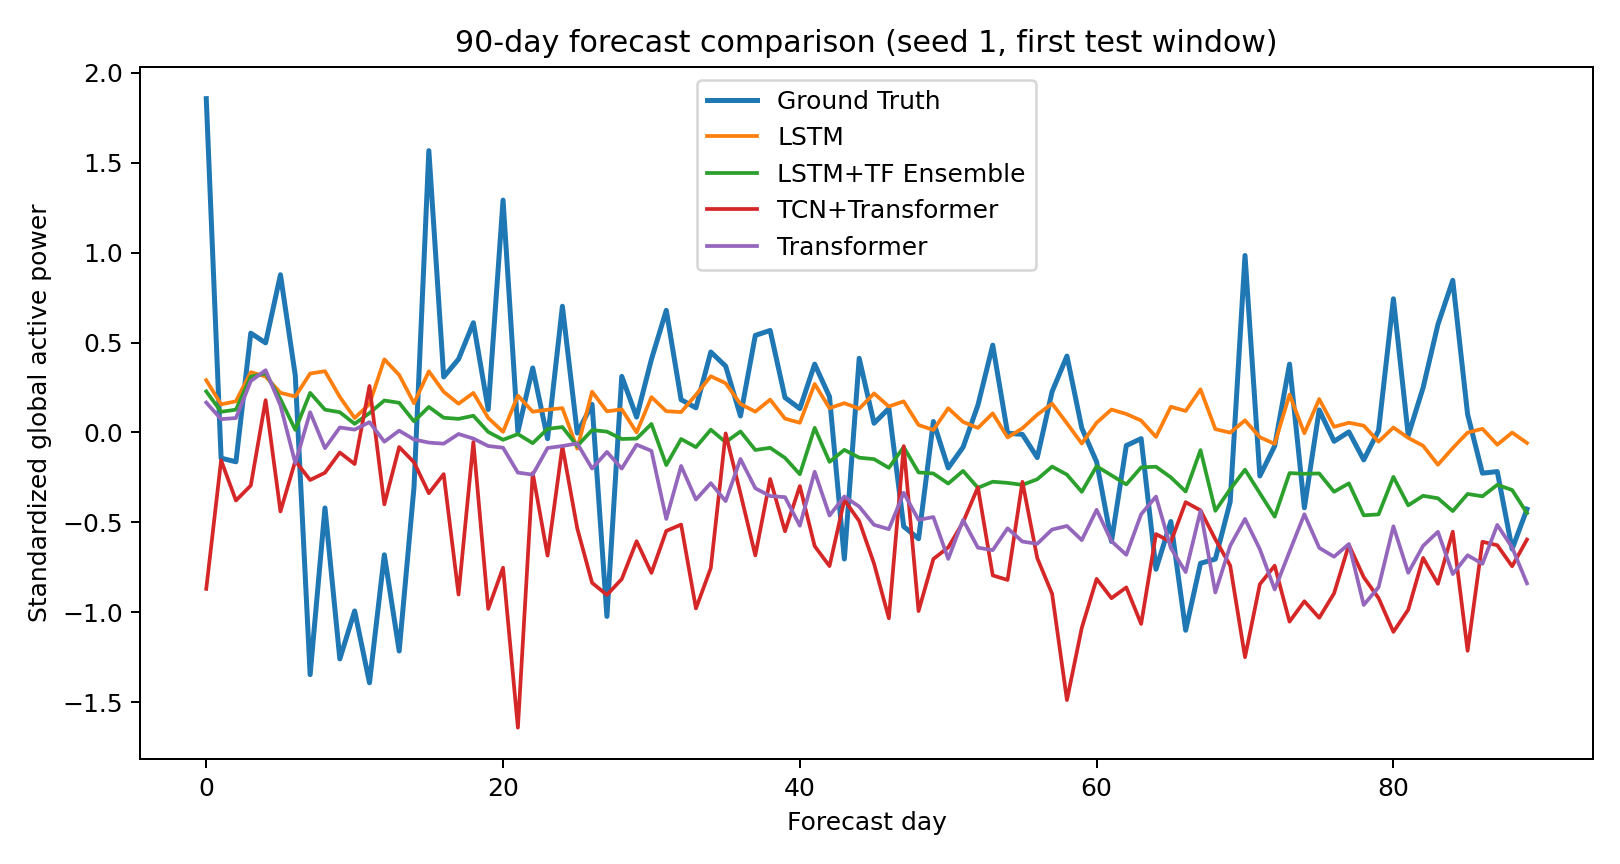
\includegraphics[width=\textwidth]{comparison_h90_seed1.png}
  \caption{Seed 1 的第一个 90 天测试窗口。Ensemble 曲线比单模型更平衡，整体误差最低，但局部峰谷仍有偏差。}
  \label{fig:h90}
\end{figure}

\begin{figure}[htbp]
  \centering
  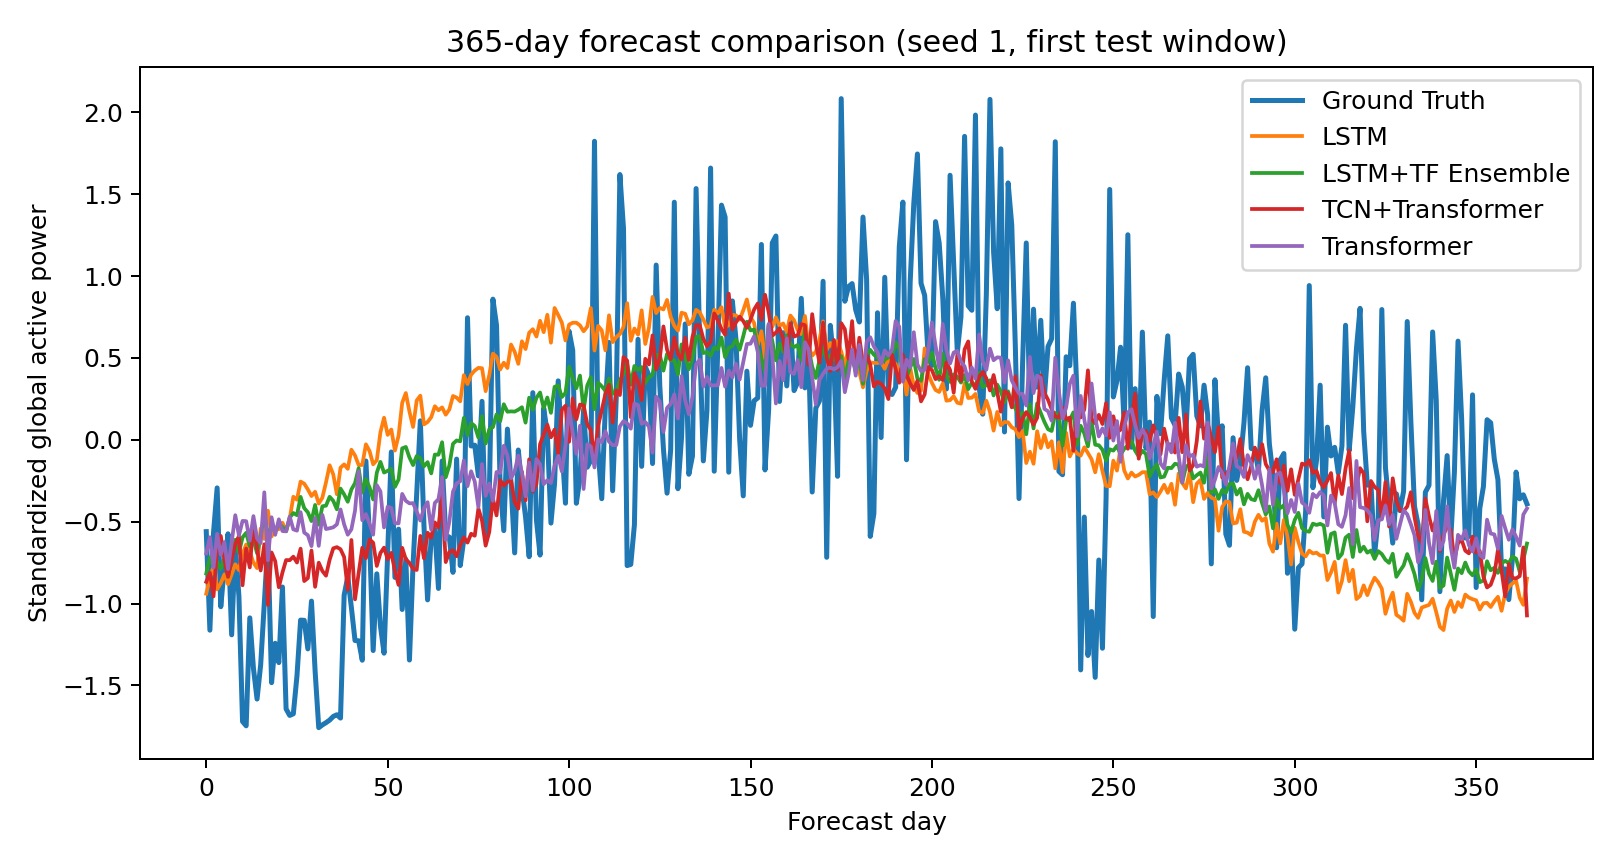
\includegraphics[width=\textwidth]{comparison_h365_seed1.png}
  \caption{Seed 1 的第一个 365 天测试窗口。长期预测更容易出现幅度收缩和趋势偏移，Ensemble 在平滑趋势与局部变化之间取得了更好的折中。}
  \label{fig:h365}
\end{figure}

\clearpage

\section{讨论}

本实验支持两个有限结论。第一，在本数据集、90 天输入窗口和当前训练预算下，单模型中 LSTM 更适合 90 天短期预测，Transformer 更适合 365 天长期预测。第二，固定等权重 LSTM+Transformer Ensemble 在两个预测窗口上都取得最低 test MSE 和 MAE，因此是当前最终改进模型。

本项目的主要限制包括：指标在标准化目标尺度上计算，便于模型比较但不直接等同于原始 kW 尺度误差；滑动窗口按窗口起点时间顺序切分，相邻样本之间存在重叠；ensemble 需要同时保留 LSTM 和 Transformer 两个模型，推理成本高于单模型；数据没有额外引入天气、节假日或住户行为特征。后续改进可以尝试反标准化指标、严格按目标日期切分、学习型 ensemble 权重，以及加入季节性和外生变量。

\subsection{有效性边界与反事实思考}

如果将评价指标反标准化到原始 kW 尺度，模型排序大概率保持一致，但误差的业务含义会更直观，也可能暴露出高负荷时段被低估的问题。如果采用更严格的目标日期切分，减少相邻窗口重叠，测试集会更难，当前数值可能上升；但这种设置更能检验跨时间段泛化。若给 TCN+Transformer 更充分的训练预算、正则化搜索或更长输入窗口，它仍可能恢复竞争力，因此本文不把它的失败解释为结构性否定，而只解释为当前数据和预算下未形成稳定收益。

从方法选择看，ensemble 的优势来自简单、可解释和不依赖测试集调权；它的代价是推理时需要维护两个基础模型。权重扫描进一步表明，horizon-specific validation tuning 并不总是可靠，尤其在 90 天预测上可能过度偏向 LSTM。若课程作业进一步追求工程简洁性，可以尝试知识蒸馏或学习一个轻量 gating 模块，把 ensemble 的互补性压缩到单模型中。若进一步追求科学严谨性，则应增加更多随机 seed、对 train/val/test 时间边界做敏感性分析，并报告原始尺度误差与标准化误差两套指标。

\section*{参考文献}
\addcontentsline{toc}{section}{参考文献}
\begin{enumerate}[leftmargin=1.4em]
  \item UCI Machine Learning Repository. Individual household electric power consumption. \href{https://archive.ics.uci.edu/dataset/235/individual+household+electric+power+consumption}{UCI 数据集页面}.
  \item Hebrail, G. and Berard, A. Individual household electric power consumption Data Set. EDF R\&D, Clamart, France, 2006--2010.
  \item Hochreiter, S. and Schmidhuber, J. Long Short-Term Memory. Neural Computation, 1997.
  \item Vaswani, A. et al. Attention Is All You Need. NeurIPS, 2017.
  \item Bai, S., Kolter, J. Z., and Koltun, V. An Empirical Evaluation of Generic Convolutional and Recurrent Networks for Sequence Modeling. arXiv, 2018.
\end{enumerate}

\section*{工具辅助说明}
\addcontentsline{toc}{section}{工具辅助说明}

本项目使用 ChatGPT/Codex 辅助进行代码实现、实验脚本整理、改进模型尝试和报告草稿生成。数据下载、清洗、训练、ensemble 评估和结果汇总均由本仓库脚本在本机环境中执行，报告表格与图像来自 \path{results/official_summary/} 中的正式实验产物。

\section*{复现与自检说明}
\addcontentsline{toc}{section}{复现与自检说明}

完整复现步骤见 \path{docs/reproducibility.md}。提交前运行自检脚本 \path{scripts/verify_submission.py}，该脚本检查 PDF 可解析性、报告必需文本、关键产物存在性，以及 \path{lstm_transformer_ensemble} 是否在 90 天和 365 天测试集 MSE/MAE 上均为第一。

\section*{最终提交检查}
\addcontentsline{toc}{section}{最终提交检查}
\begin{itemize}[leftmargin=1.4em]
  \item PDF 报告：\path{reports/ML_homework_report.pdf}
  \item LaTeX 报告源稿：\path{reports/ML_homework_report.tex}
  \item Markdown 报告源稿：\path{reports/ML_homework_report.md}
  \item 复现说明：\path{docs/reproducibility.md}
  \item 提交自检：\path{scripts/verify_submission.py}
  \item GitHub 链接：\href{https://github.com/ziangbuchu/ML_homework}{https://github.com/ziangbuchu/ML\_homework}
  \item 提交入口：\href{https://docs.qq.com/form/page/DT3pqV3pNcGV6TG1z}{https://docs.qq.com/form/page/DT3pqV3pNcGV6TG1z}
  \item 截止时间：2026 年 7 月 15 日中午 12:00 前
\end{itemize}

\end{document}
